\documentclass[fleqn]{beamer}
\beamertemplatenavigationsymbolsempty

\usepackage[T1]{fontenc}
\usepackage[utf8]{inputenc}

\usepackage{amsmath,amssymb}
\usepackage{graphicx}
\usepackage{mathptmx}
\usepackage{subcaption}
\usepackage{amsthm}
\usepackage{tikz}
%\usepackage[colorlinks=true,naturalnames=true,plainpages=false,pdfpagelabels=true]{hyperref}
\usetikzlibrary{patterns,decorations.pathmorphing,positioning, arrows, chains}

\usepackage[backend=biber, sorting=none]{biblatex}
\addbibresource{uni.bib}

\setbeamertemplate{endpage}{%
    \begin{frame}
        \centering
        \Large \emph{To be continued\ldots}

        \vspace{1cm}

        \centering
        \Large \emph{Thank You!}
    \end{frame}
}

\AtEndDocument{\usebeamertemplate{endpage}}

% vertical separator macro
\newcommand{\vsep}{
  \column{0.0\textwidth}
    \begin{tikzpicture}
      \draw[very thick,black!10] (0,0) -- (0,7.3);
    \end{tikzpicture}
}
\setlength{\mathindent}{0pt}

% Beamer theme
\usetheme{UniVienna}
\usefonttheme[onlysmall]{structurebold}
\mode<presentation>
\setbeamercovered{transparent=10}

\title
{Complex Network Analysis}
\subtitle{Seminar, Project}
\author[Popović Milutin]
{Popović Milutin}
\date{17. March 2021}

\begin{document}
    \begin{frame}
        \titlepage
    \end{frame}

    \begin{frame}
        \begin{figure}[H]
            \centering
            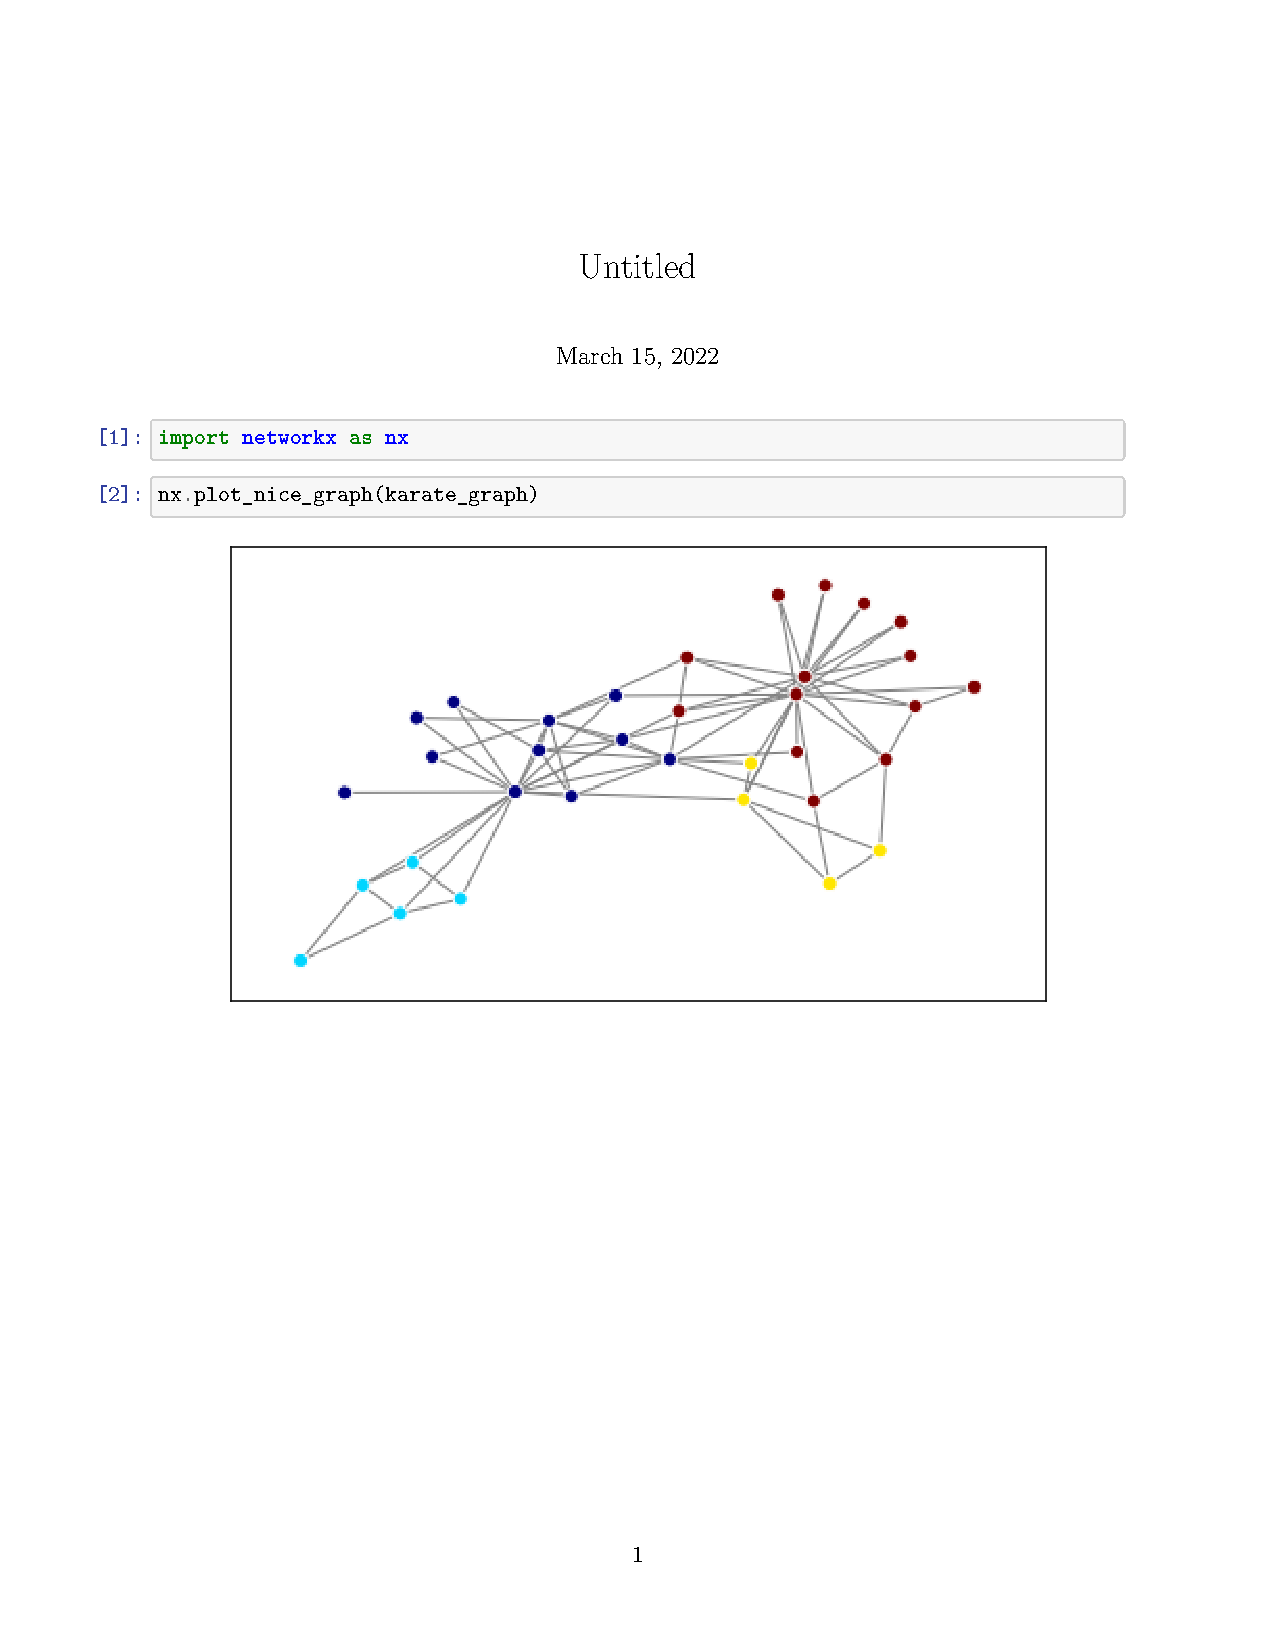
\includegraphics[width=1.1\textwidth,
                             clip,
                             trim=0cm 10cm 0cm 7cm]
                             {./pics/code_example.pdf}
        \end{figure}
    \end{frame}

    \begin{frame}
        \centering
        \texttt{\$ pip install networkx}
        \vspace{1cm}
    \end{frame}

    \begin{frame}
        \centering
        \texttt{\$ pip install networkx}
        \vspace{1cm}
        \begin{itemize}
            \item[$\to$] Go to PyPi (Python Package Index) and download \&
                install \texttt{networkx}
        \end{itemize}
    \end{frame}

    \begin{frame}
        \begin{figure}[H]
            \centering
            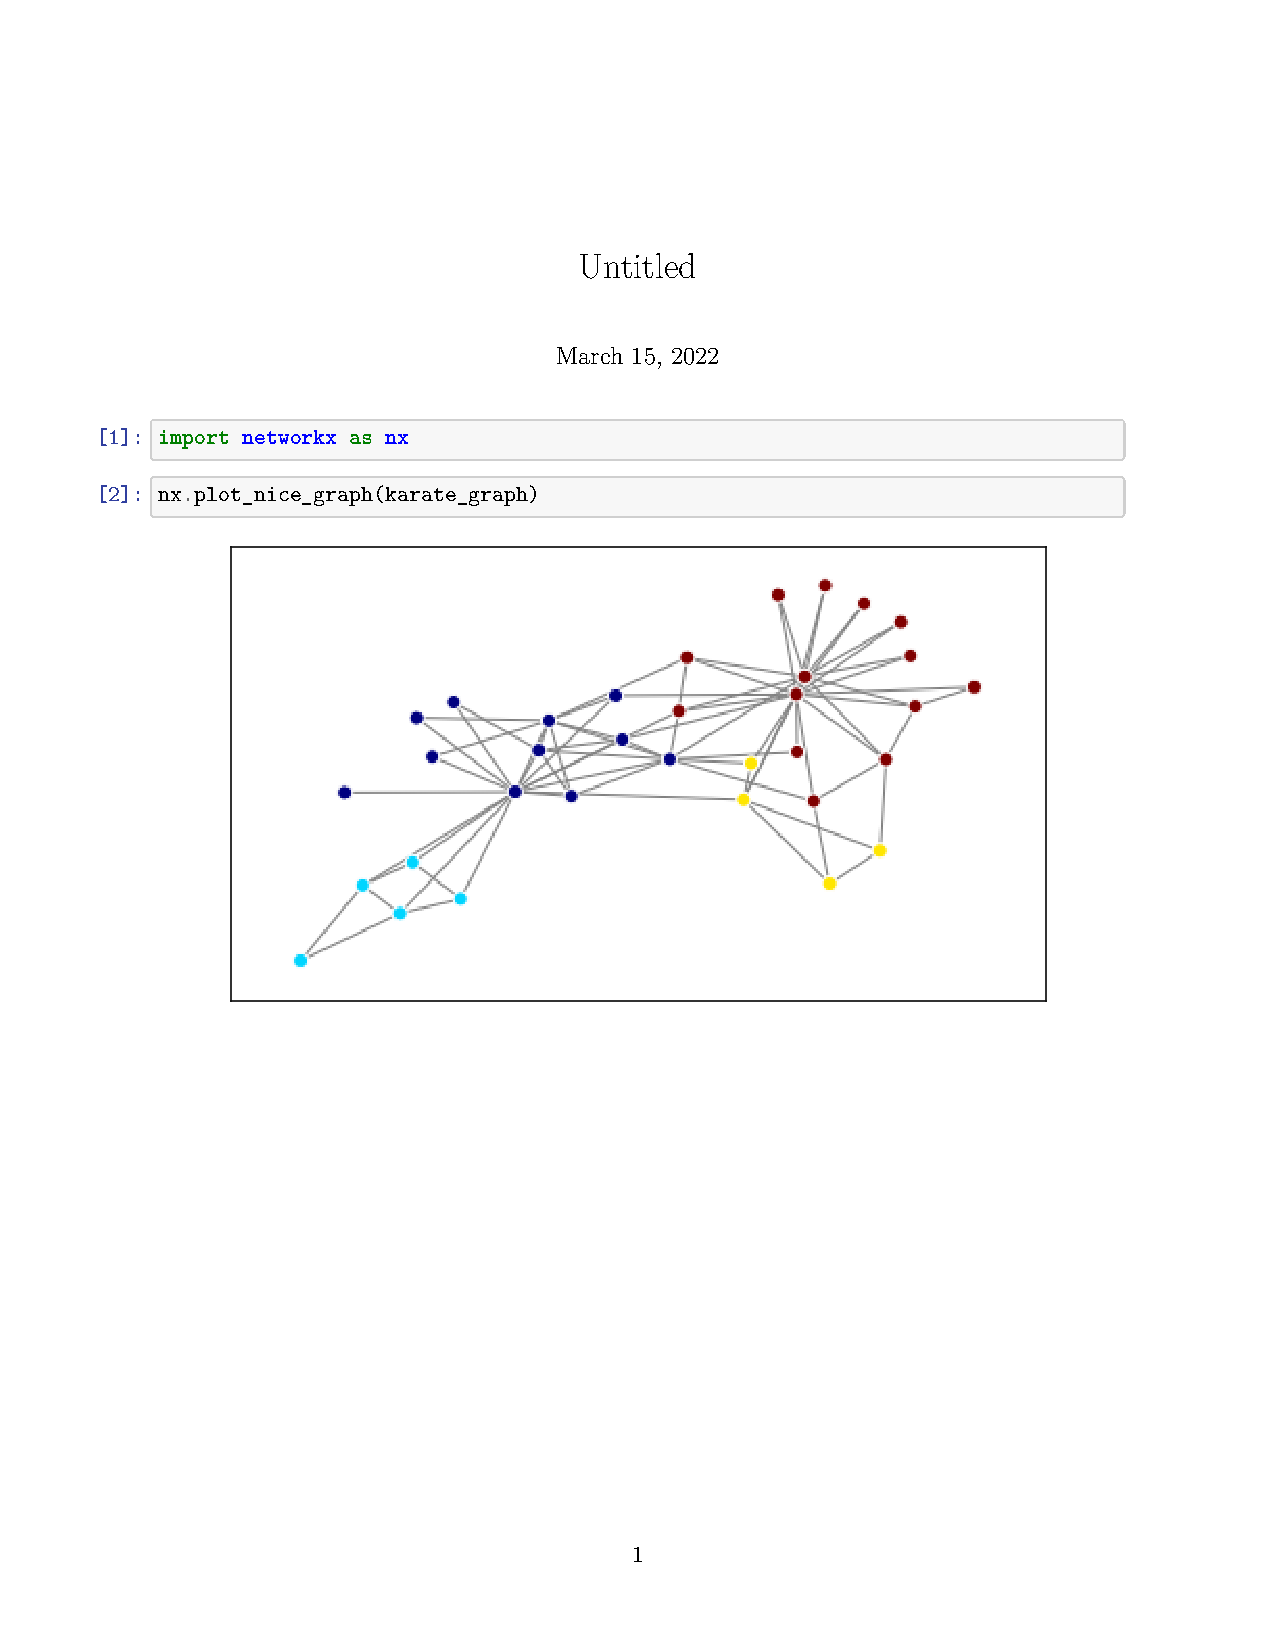
\includegraphics[width=1.1\textwidth,
                             clip,
                             trim=0cm 10cm 0cm 7cm]
                             {./pics/code_example.pdf}
        \end{figure}
    \end{frame}

    \begin{frame}
        \begin{figure}[H]
            \centering
            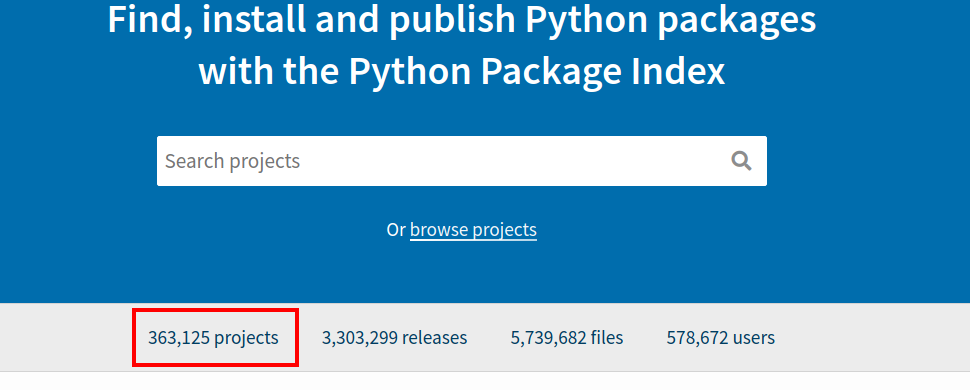
\includegraphics[width=0.8\textwidth]
                             {./pics/pypi.png}
        \end{figure}
    \end{frame}

    \begin{frame}
        \begin{columns}[T]
            \column{0.4\textwidth}
        \begin{align*}
            \text{Nodes}\ &\to\  \text{Repositories}\\
            \text{Edges}\ &\to\ \text{Requirements}(Imoprts)
        \end{align*}
        \end{columns}
    \end{frame}

    \begin{frame}
        \begin{columns}[T]
        \centering
            \column{0.4\textwidth}
        \begin{block}{\centering Directed Graph}
            \centering \texttt{scipy $\to$ numpy}\\
        \end{block}
        \end{columns}
    \end{frame}

    \begin{frame}
        \begin{columns}[T]
        \centering
            \column{0.4\textwidth}
        \begin{block}{\centering Directed Graph}
            \centering \texttt{scipy $\to$ numpy}\\
            \centering \texttt{scipy $\not\gets$ numpy}
        \end{block}
        \end{columns}
    \end{frame}

    \begin{frame}
        \centering
        \texttt{DiGraph with 361,742 nodes and 719,797 edges}\\
        \vspace{1cm}
    \end{frame}

    \begin{frame}
        \centering
        \texttt{DiGraph with 361,742 nodes and 719,797 edges}\\
        \vspace{1cm}
        \begin{itemize}
            \item[$\to$]\centering $\sim$362,000 out of $\sim$363,000  (Not what I expected)!
        \end{itemize}
    \end{frame}

    \begin{frame}
        \centering
        \texttt{DiGraph with 361,742 nodes and 719,797 edges}\\
        \vspace{1cm}
        \begin{itemize}
            \item[$\to$]\centering $\sim$362,000 out of $\sim$363,000  (Not what I expected)!
            \item[$\to$]\centering Significant data has $k_i > 0$ $\to$
                               $\sim$164,000 nodes and $\sim$720,000 edges
        \end{itemize}
    \end{frame}

    \begin{frame}
        \frametitle{Plotting Dependencies}
    \begin{figure}[htpb]
        \centering
        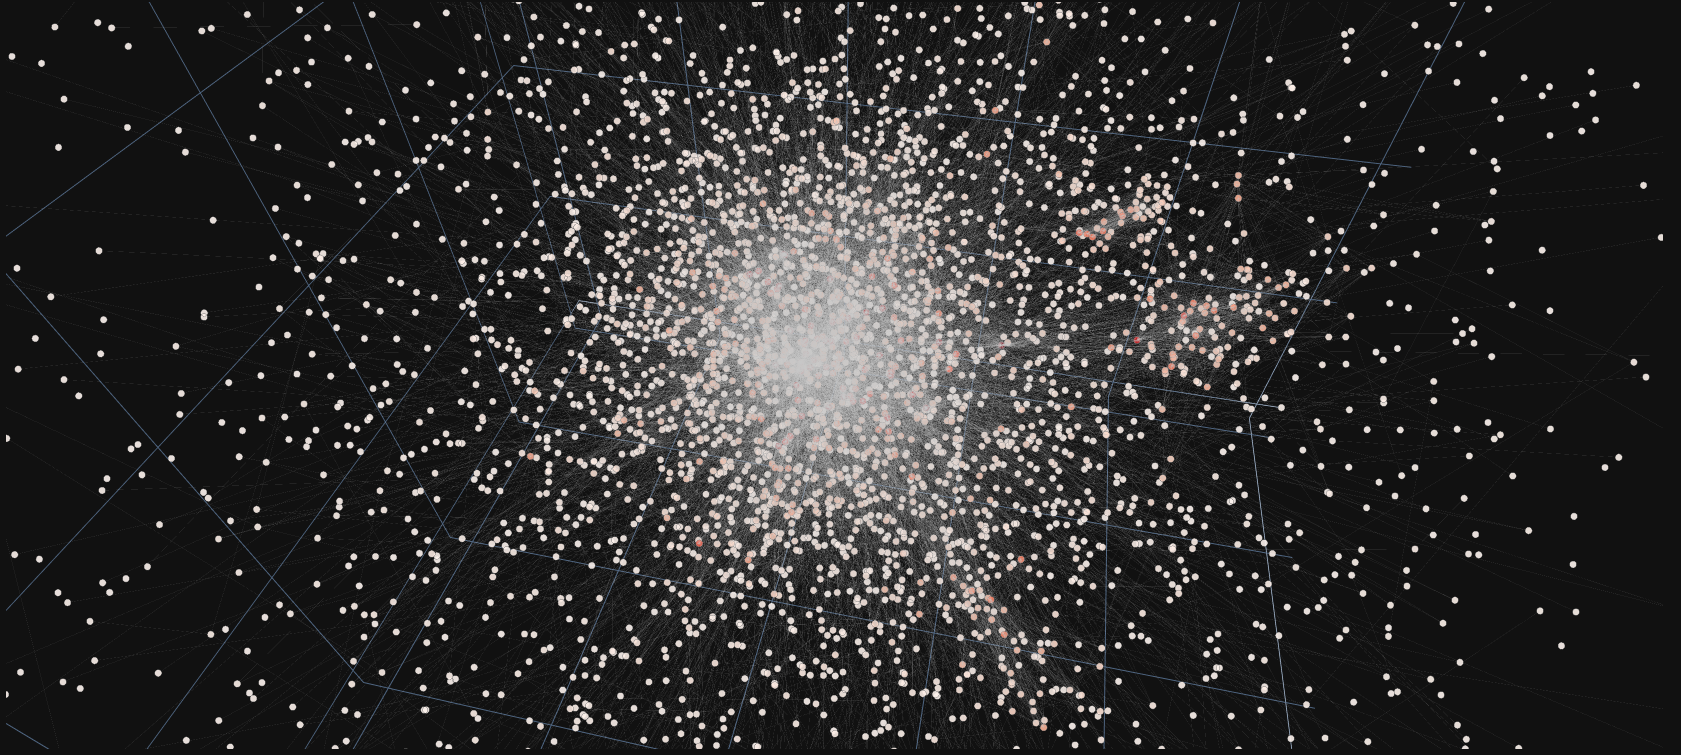
\includegraphics[width=1\textwidth, ]{./pics/req_3d.png}
        \caption{Plot of the Python Dependencies Network $k_{\text{in}}\ge
            10$, $N=4826$, $L=20847$
            (red nodes indicate high degree)}
    \end{figure}
    \end{frame}

    \begin{frame}
        \frametitle{Network Information}
      \begin{columns}[T]
        \column{0.4\textwidth}
            \begin{block}{\centering Basic Properties}
                \begin{align*}
                   \quad\qquad \langle k_{\text{in}}\rangle  &= 1.99\\
                   \quad\qquad \langle k_{\text{out}}\rangle  &= 1.99\\
                   \quad\qquad \langle k\rangle  &= 8.75\\
                   \quad\qquad \langle k^2\rangle  &=\ -
                \end{align*}
          \end{block}

        \column{0.54\textwidth}
        \begin{block}{\centering Specific Properties}
                \begin{align*}
                    S &\simeq 1 \hspace{1.7cm} Connected\\
                      \langle d_\text{min}\rangle  &= 7.63 \qquad
                      \text{Small-World}\\
                      d_{\text{max}} &= 18.09\\
                      r &= -0.125 \qquad \text{Assortative}\\
                \end{align*}
        \end{block}
        \end{columns}
    \end{frame}

    \begin{frame}
        \frametitle{Undirected Degree Distribution}
    \begin{figure}[htpb]
        \centering
        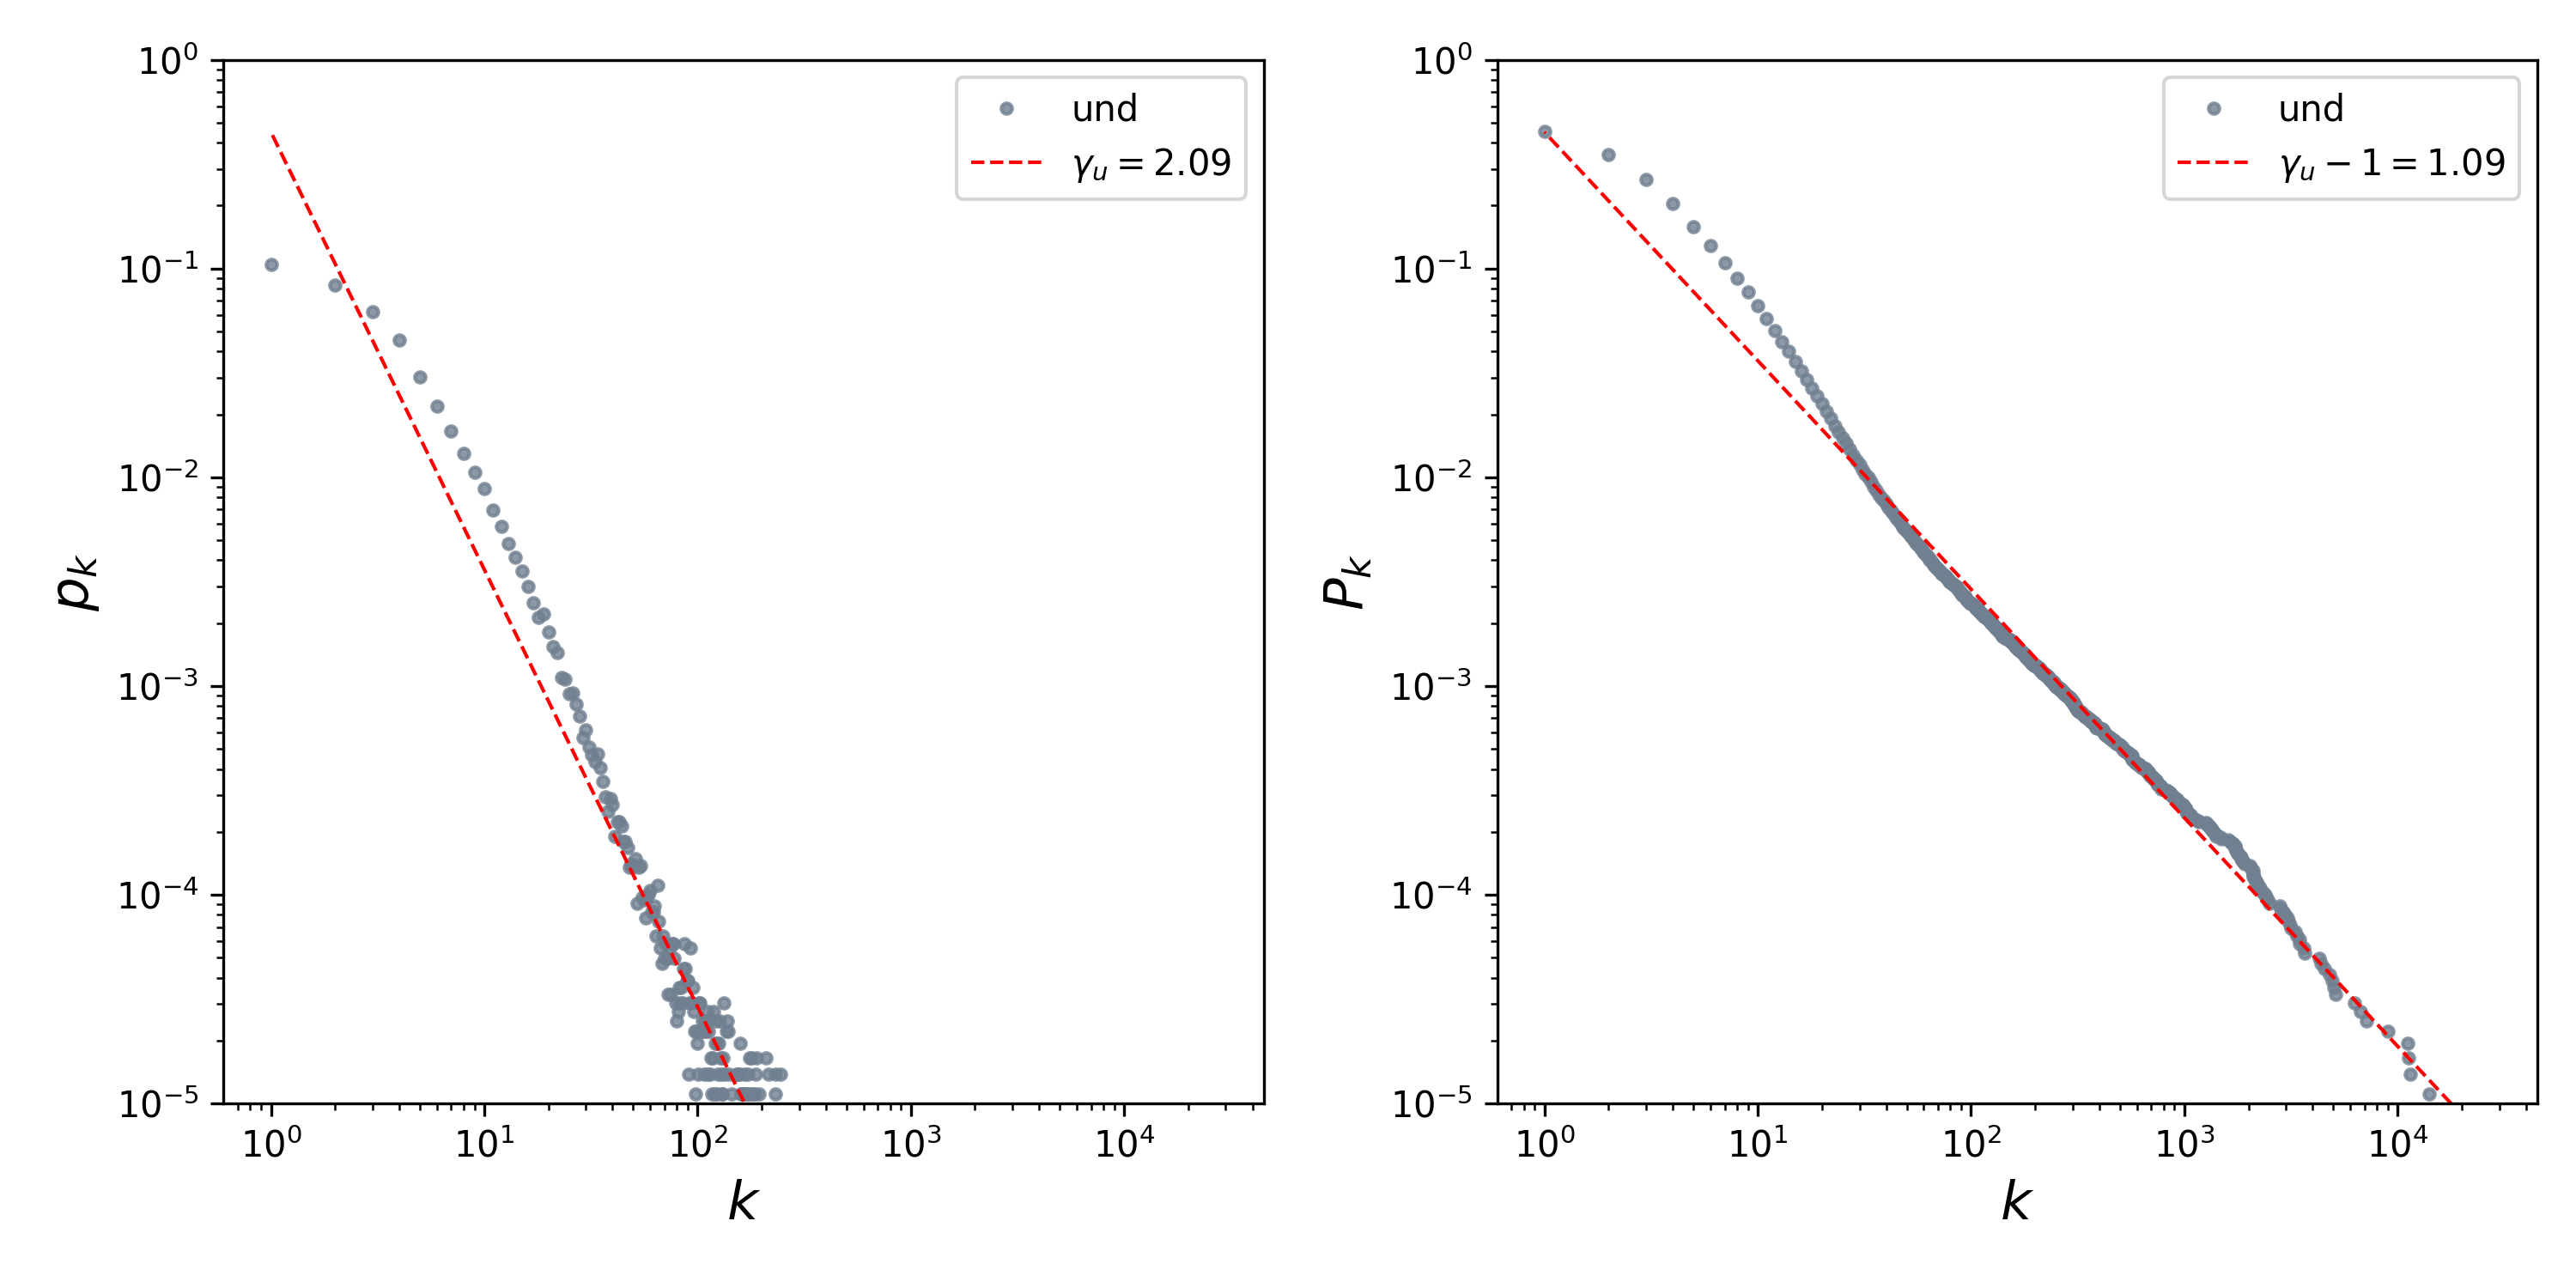
\includegraphics[width=1\textwidth]{./pics/dist_u.png}
        \caption{Undirected (left) distribution $p_k$ (right) cumulative
        degree distribution with fit for $k > 0$}
    \end{figure}
    \end{frame}

    \begin{frame}
        \frametitle{Directed Degree Distribution}
    \begin{figure}[htpb]
        \centering
        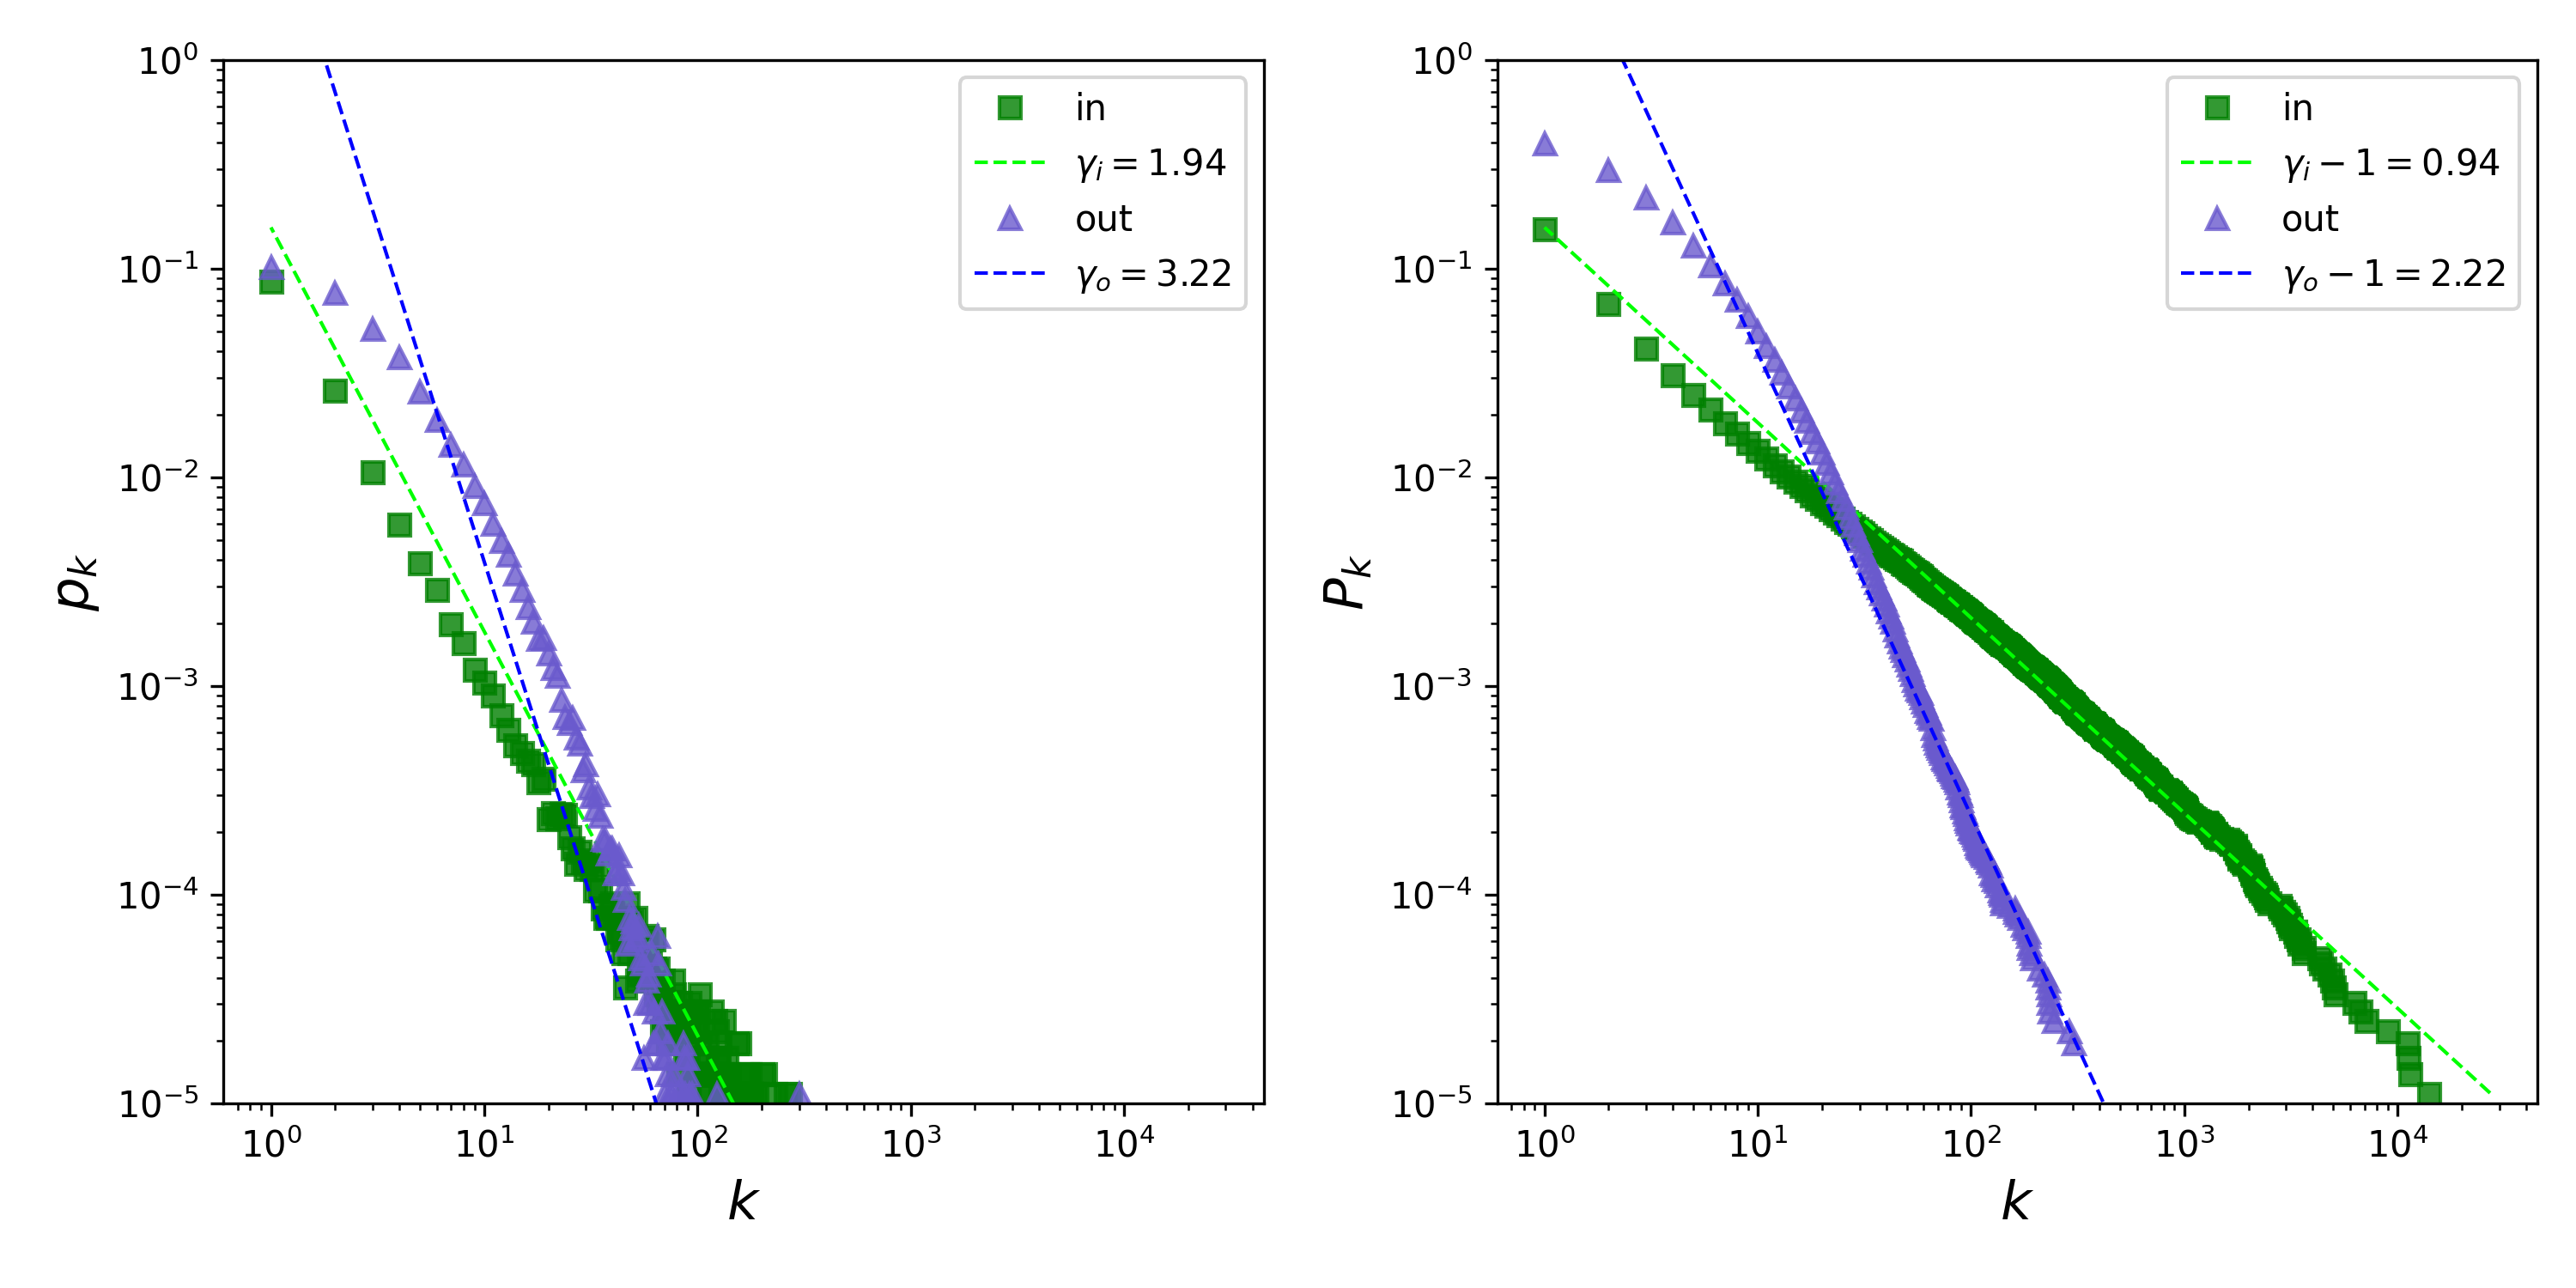
\includegraphics[width=1\textwidth]{./pics/dist_d.png}
        \caption{Directed (left) distribution $p_k$ (right) cumulative
        degree distribution with fit for $k > 0$}
    \end{figure}
    \end{frame}

    \begin{frame}
        \frametitle{Community Detection}
        \begin{columns}[T]
        \column{0.4\textwidth}
        \begin{block}{\centering Louvain-Algorithm}
            \centering
            Optimize \textbf{Modularity} $M$\\
            $O(L)$
        \end{block}
        \column{0.4\textwidth}
        \begin{block}{\centering Info-Map-Algorithm}
            \centering
            Optimize \textbf{Map-Equation} $\mathcal{L}$\\
            $O(N\log(N))$
        \end{block}
        \end{columns}
        \vspace{1cm}
    \end{frame}

    \begin{frame}
        \frametitle{Community Detection}
        \begin{columns}[T]
        \column{0.4\textwidth}
        \begin{block}{\centering Louvain-Algorithm}
            \centering
            Optimize \textbf{Modularity} $M$\\
            $O(N)$
        \end{block}
        \column{0.4\textwidth}
        \begin{block}{\centering Info-Map-Algorithm}
            \centering
            Optimize \textbf{Map-Equation} $\mathcal{L}$\\
            $O(N\log(N)$
        \end{block}
        \end{columns}
        \vspace{1cm}
        \begin{itemize}
            \item[$\to$]\centering Detect \& Analyze Community Structure
        \end{itemize}
    \end{frame}

    \begin{frame}
        \frametitle{Sneak Preview}
        \begin{figure}[htpb]
            \centering
            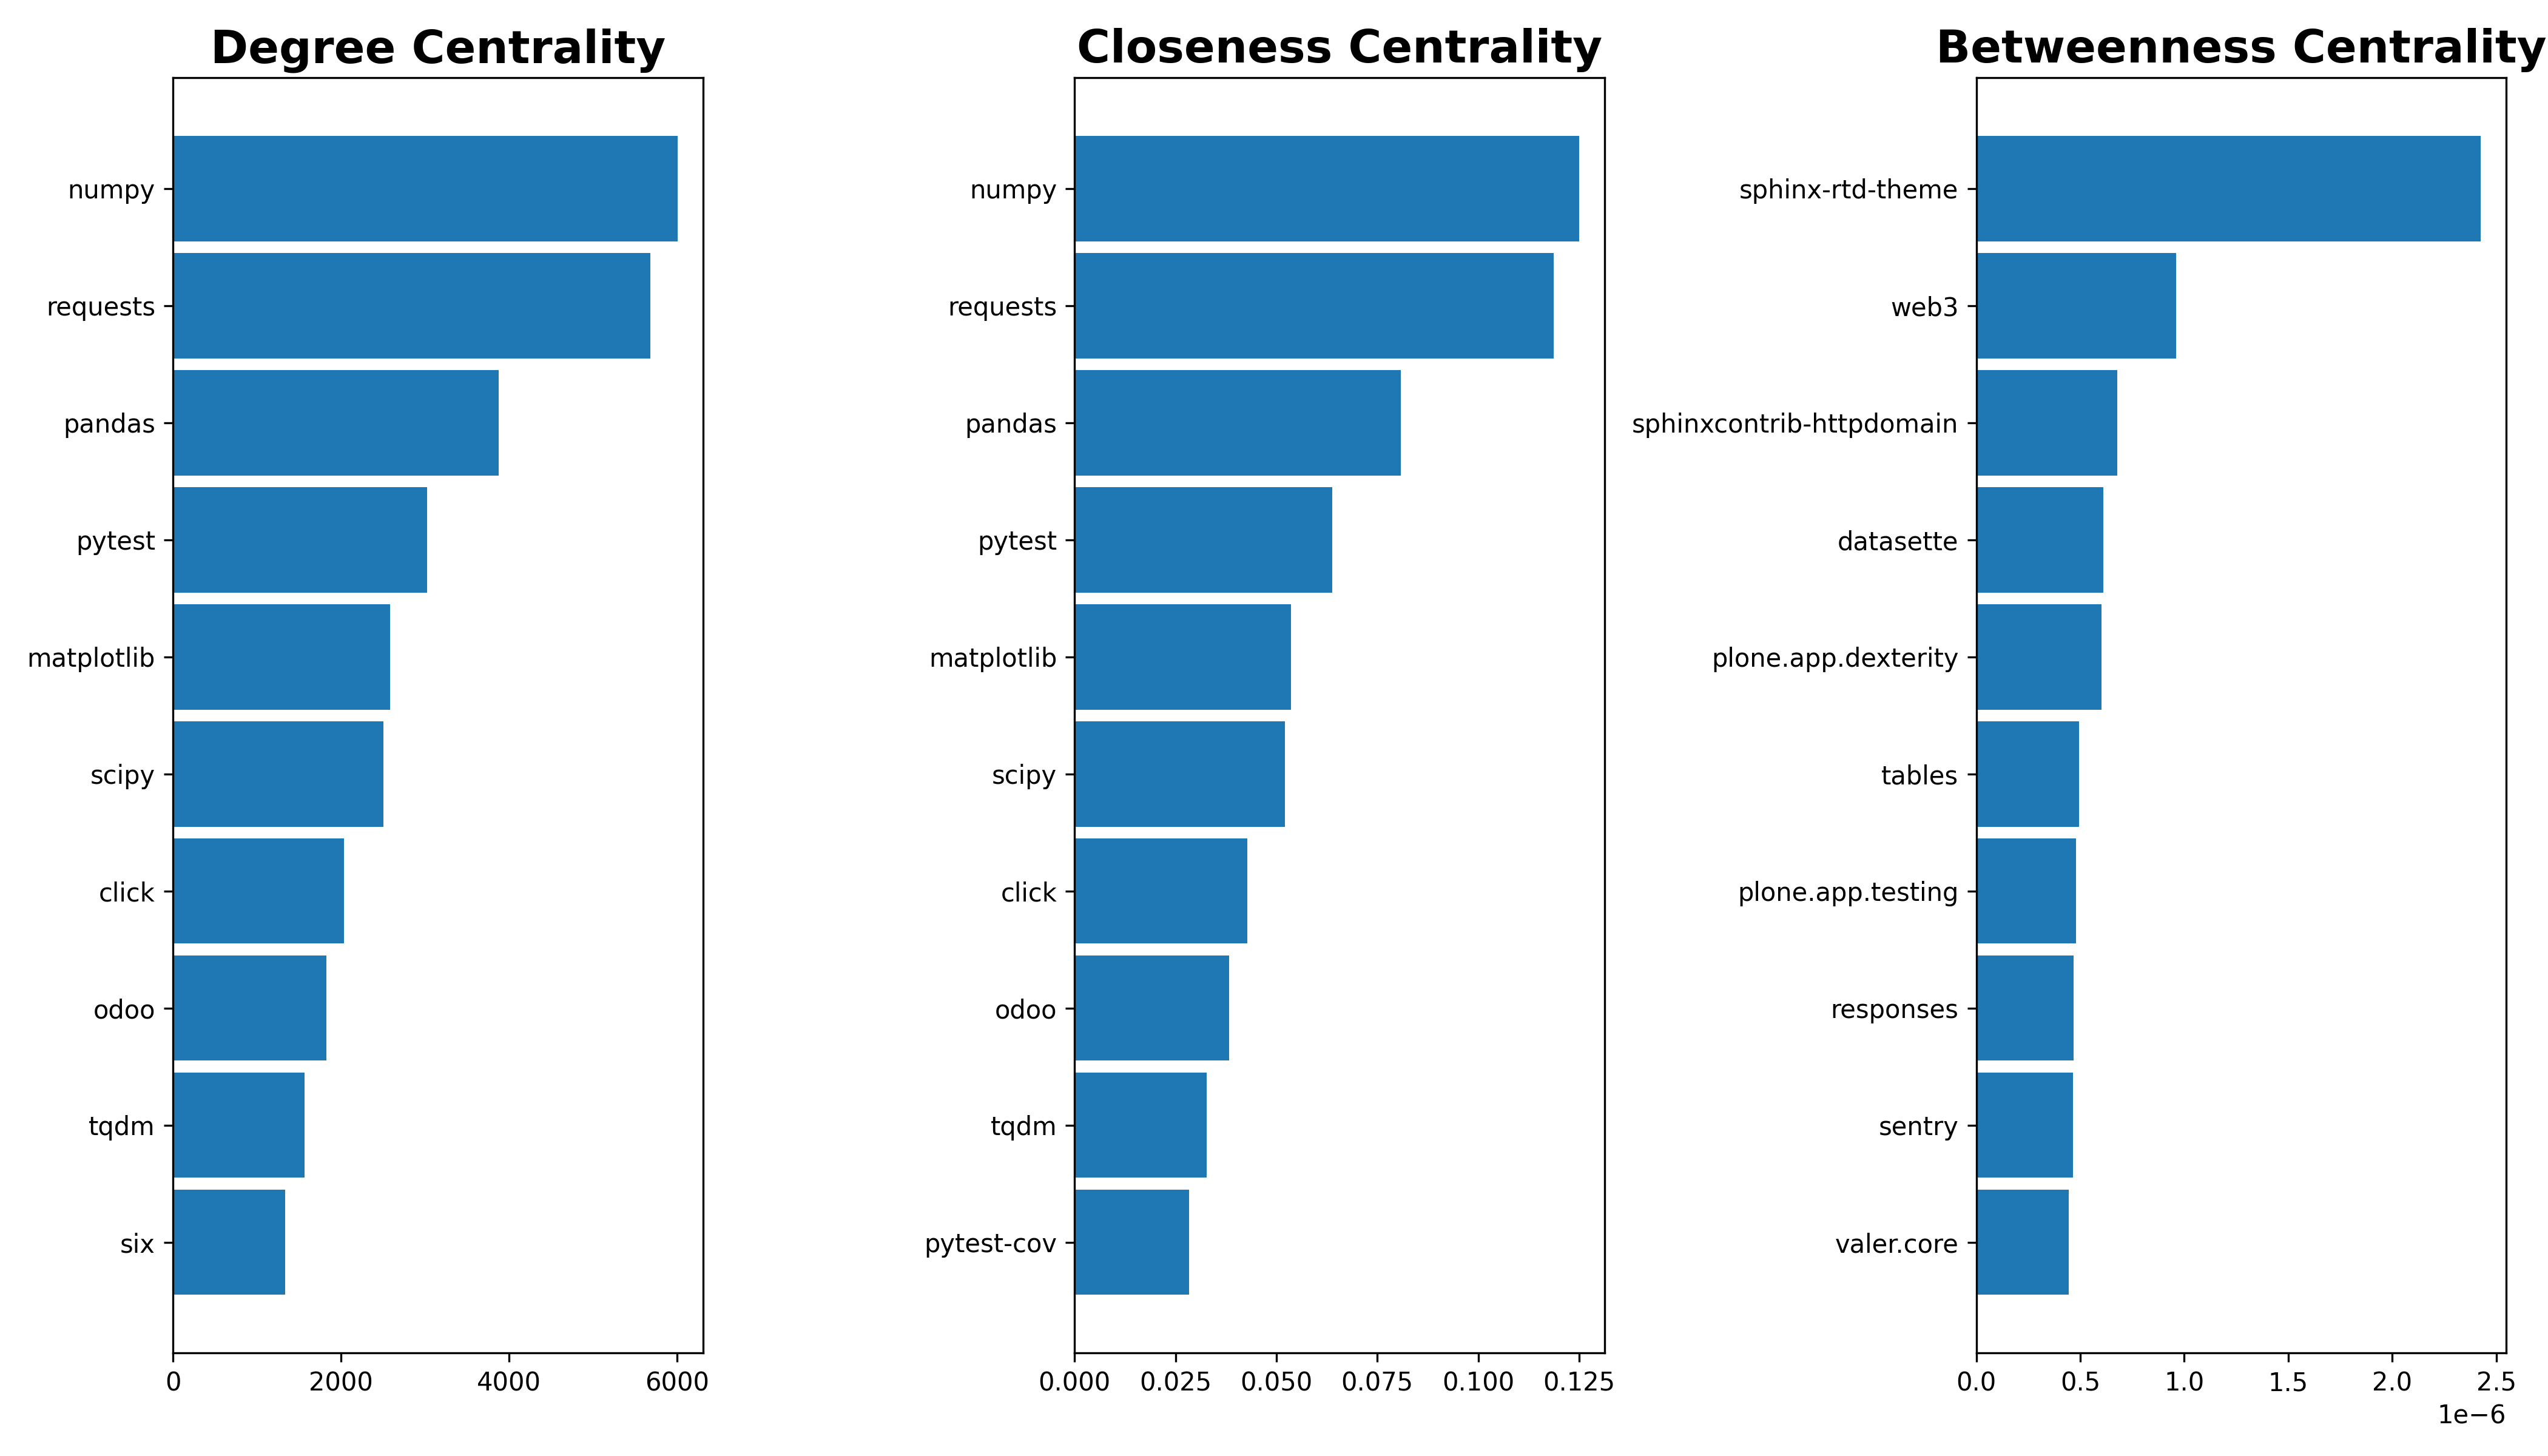
\includegraphics[width=1\textwidth]{./pics/sneak_peak.png}
            \label{fig:-frac-pics-sneap_peak-png}
        \end{figure}
    \end{frame}

    \begin{frame}{Bibliography}
        \nocite{barabasi}
        \nocite{motivation}
        \nocite{pypi}
        \printbibliography
    \end{frame}
\end{document}

